\section{System and Raspberry Pi specifications}

The following setup was used to collect results and benchmarking data:

\begin{table}[htbp]
	\centering
	\begin{tabular}{@{}lccc@{}}
		\toprule
		\textbf{Specification} & \textbf{Desktop} & \textbf{RPI5} & \textbf{RPI4} \\ 
		\midrule
		Processor             & AMD Ryzen 7 5800H & Cortex A-76 & Cortex A-72 \\
		Processor Type        & x86               & ARM         & ARM \\
		Cores/Threads         & 8/16              & 4/4         & 4/4 \\
		RAM Size              & 16GB              & 8GB         & 4GB \\
		RAM Type/Speed        & DDR4 / 3200 MT/s  & LPDDR4/ 4267 MT/s & LPDDR4 / 3200 MT/s \\
		Operating System      & Ubuntu Linux 22.04.4 LTS & Debian GNU/Linux 12 (bookworm) &  \\
		GCC Compiler          & 11.4.0            & 12.2.0      &  \\
		GNAT Compiler         & 10.5.0            & 12.2.0      &  \\
		Java Compiler         & 11.0.22           & 17.0.10     &  \\
		C\# (.NET SDK)        & 7.0.117           & 6.0.101     &  \\
		\bottomrule
	\end{tabular}
	\caption{Specifications and Software Versions of Desktop and Raspberry Pi Systems}
	\label{tab:spec_comparisons}
\end{table}

\section{Objective 1: \texttt{mpbenchmark}}

Profiling results using \texttt{Valgrind/Calgrind} are shown in figure ~\ref{fig:mpbenchmark_profiled}.

\begin{figure}[H] % Positioning preference: here, top, bottom, page
	\centering
	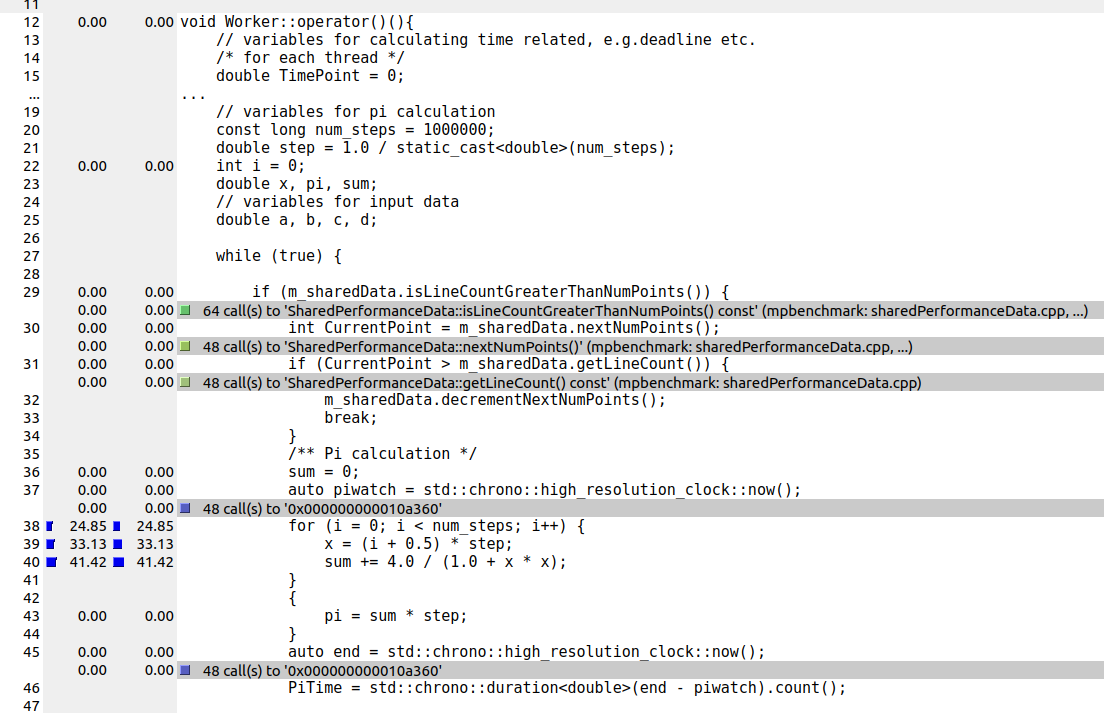
\includegraphics[width=1\textwidth, height=20cm]{~/Documents/Part_D_Modules/Individual_Project/Individual_report/figures/valgrind_mpbenchmark.png} % Adjust the path and width as needed
	\caption{\texttt{Calgrind} profiling results on the \texttt{mpbenchmark} application. Ir - Instruction Fetch, CEst - Cycle estimation.}
	\label{fig:mpbenchmark_profiled} % Use this label to reference the figure
\end{figure} 

Code for implementing the approximation of $\pi$ using single and double point floating precision with \texttt{NEON} instructions are shown in listings ~\ref{lst:neon_float} and ~\ref{lst:neon_double}.

\begin{lstlisting}[
	caption={Approximation of $\pi$ using single point precision \texttt{NEON} instructions.},
	label={lst:neon_float}
	]
double Worker::approximatePi(){
	double pi = 0.0;
	static constexpr long num_steps = 1000000;
	static constexpr double step = 1.0 / static_cast<double>(num_steps);
	
	#if defined(__AVX2__)
	// Insert AVX2 specific code here ...

	#elif defined(__ARM_NEON)
	// Insert NEON specific code here
	float32_t f_step = 1.0f / static_cast<float32_t>(num_steps); // Using float for NEON
	float32x4_t vec_step = vdupq_n_f32(f_step);
	float32x4_t vec_half_step = vdupq_n_f32(0.5f * f_step);
	float32x4_t vec_one = vdupq_n_f32(1.0f);
	float32x4_t vec_four = vdupq_n_f32(4.0f);
	float32_t sum = 0.0f; // Using float for NEON
	
	for (int i = 0; i < num_steps; i += 4) {
		float32x4_t vec_i = vsetq_lane_f32(i + 3, vsetq_lane_f32(i + 2, vsetq_lane_f32(i + 1, vsetq_lane_f32(i, vdupq_n_f32(0.0f), 0), 1), 2), 3);
		float32x4_t vec_x = vaddq_f32(vmulq_f32(vec_i, vec_step), vec_half_step);
		float32x4_t vec_temp = vdivq_f32(vec_four, vaddq_f32(vec_one, vmulq_f32(vec_x, vec_x)));
		sum += vaddvq_f32(vec_temp); // Horizontal sum of vector elements
	}
	
	pi = sum * f_step;
	#else
	// Insert regular code here ...
	#endif
	return pi;
}
\end{lstlisting}


\begin{lstlisting}[
	caption={Approximation of $\pi$ using double point precision \texttt{NEON} instructions.},
	label={lst:neon_double}
	]
	double Worker::approximatePi(){
		double pi = 0.0;
		static constexpr long num_steps = 1000000;
		static constexpr double step = 1.0 / static_cast<double>(num_steps);
		
		#if defined(__AVX2__)
		// Insert AVX2 specific code here ...
		
		#elif defined(__ARM_NEON)
		// Insert NEON specific code here
		float64x2_t vec_step = vdupq_n_f64(step);
		float64x2_t vec_half_step = vdupq_n_f64(0.5 * step);
		float64x2_t vec_one = vdupq_n_f64(1.0);
		float64x2_t vec_four = vdupq_n_f64(4.0);
		float64_t sum = 0.0;
		
		for (int i = 0; i < num_steps; i += 2) {
			// Since direct lane setting for float64x2_t via intrinsics like vsetq_lane_f64 isn't straightforward,
			// We compute x and its index scalarly and then load them into vectors.
			double x0 = (i + 0.5) * step;
			double x1 = (i + 1.5) * step;
			float64x2_t vec_x = {x0, x1}; // Directly initialize the vector with double values.
			
			float64x2_t vec_temp = vdivq_f64(vec_four, vaddq_f64(vec_one, vmulq_f64(vec_x, vec_x)));
			sum += vaddvq_f64(vec_temp); // Horizontal sum of vector elements.
		}
		
		pi = sum * step;
		#else
		// Insert regular code here ...
		#endif
		return pi;
	}
\end{lstlisting}

To use \texttt{AVX2} instructions for the application, the following changes were made to the \texttt{CMakeLists.txt} file, however no changes were required to use \texttt{NEON} instructions, see listing ~\ref{lst:cmake_simd}.

\begin{lstlisting}[
	language=bash,
	caption={Adding \texttt{-mavx2 -mfma} flags to the \texttt{CMake} file to allow the project to use \texttt{AVX2} instructions.},
	label={lst:cmake_simd}
	]
	# Compiler optimizations
	include(CheckCXXCompilerFlag)
	
	# Check and enable AVX2 and FMA for x86_64 architecture
	CHECK_CXX_COMPILER_FLAG("-mavx2" COMPILER_SUPPORTS_AVX2)
	CHECK_CXX_COMPILER_FLAG("-mfma" COMPILER_SUPPORTS_FMA)
	if (COMPILER_SUPPORTS_AVX2 AND COMPILER_SUPPORTS_FMA)
	target_compile_options(${PROJECT_NAME} PRIVATE -mavx2 -mfma)
	endif()
	
	if (CMAKE_SYSTEM_PROCESSOR MATCHES "arm" OR CMAKE_SYSTEM_PROCESSOR MATCHES "aarch64")
	# For ARMv8-A (aarch64), NEON is always available. No need for -mfpu=neon
	# We can set architecture-specific flags if necessary, but for NEON, it's not required.
	endif
\end{lstlisting}

Results collected from Raspberry Pi 4 can be seen in figures ~\ref{fig:mpbenchmark_rpi4_plot} and ~\ref{fig:mpbenchmark_rpi4_speedup_plot}. 

\begin{figure}[H] % Positioning preference: here, top, bottom, page
	\centering
	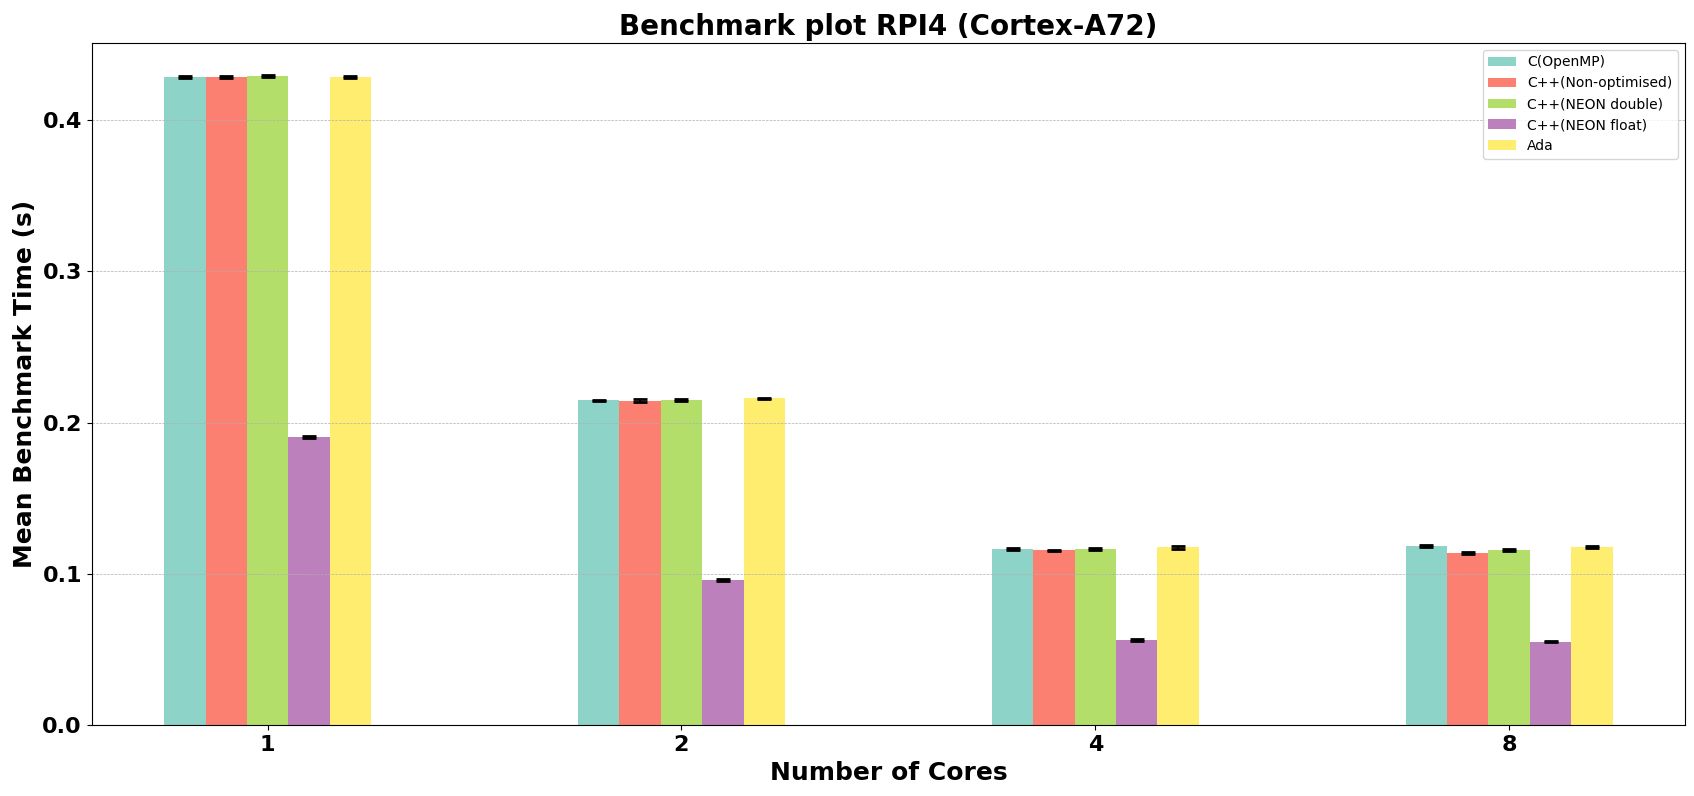
\includegraphics[width=1\textwidth, height=20cm]{~/Documents/Part_D_Modules/Individual_Project/Individual_report/figures/mpbenchmark_rpi4.png} % Adjust the path and width as needed
	\caption{Mean benchmark plot of results collected from Raspberry Pi 4(in seconds). The error bars represent 95\% confidence interval. (Lower is better).}
	\label{fig:mpbenchmark_rpi4_plot} % Use this label to reference the figure
\end{figure}

\begin{figure}[H] % Positioning preference: here, top, bottom, page
	\centering
	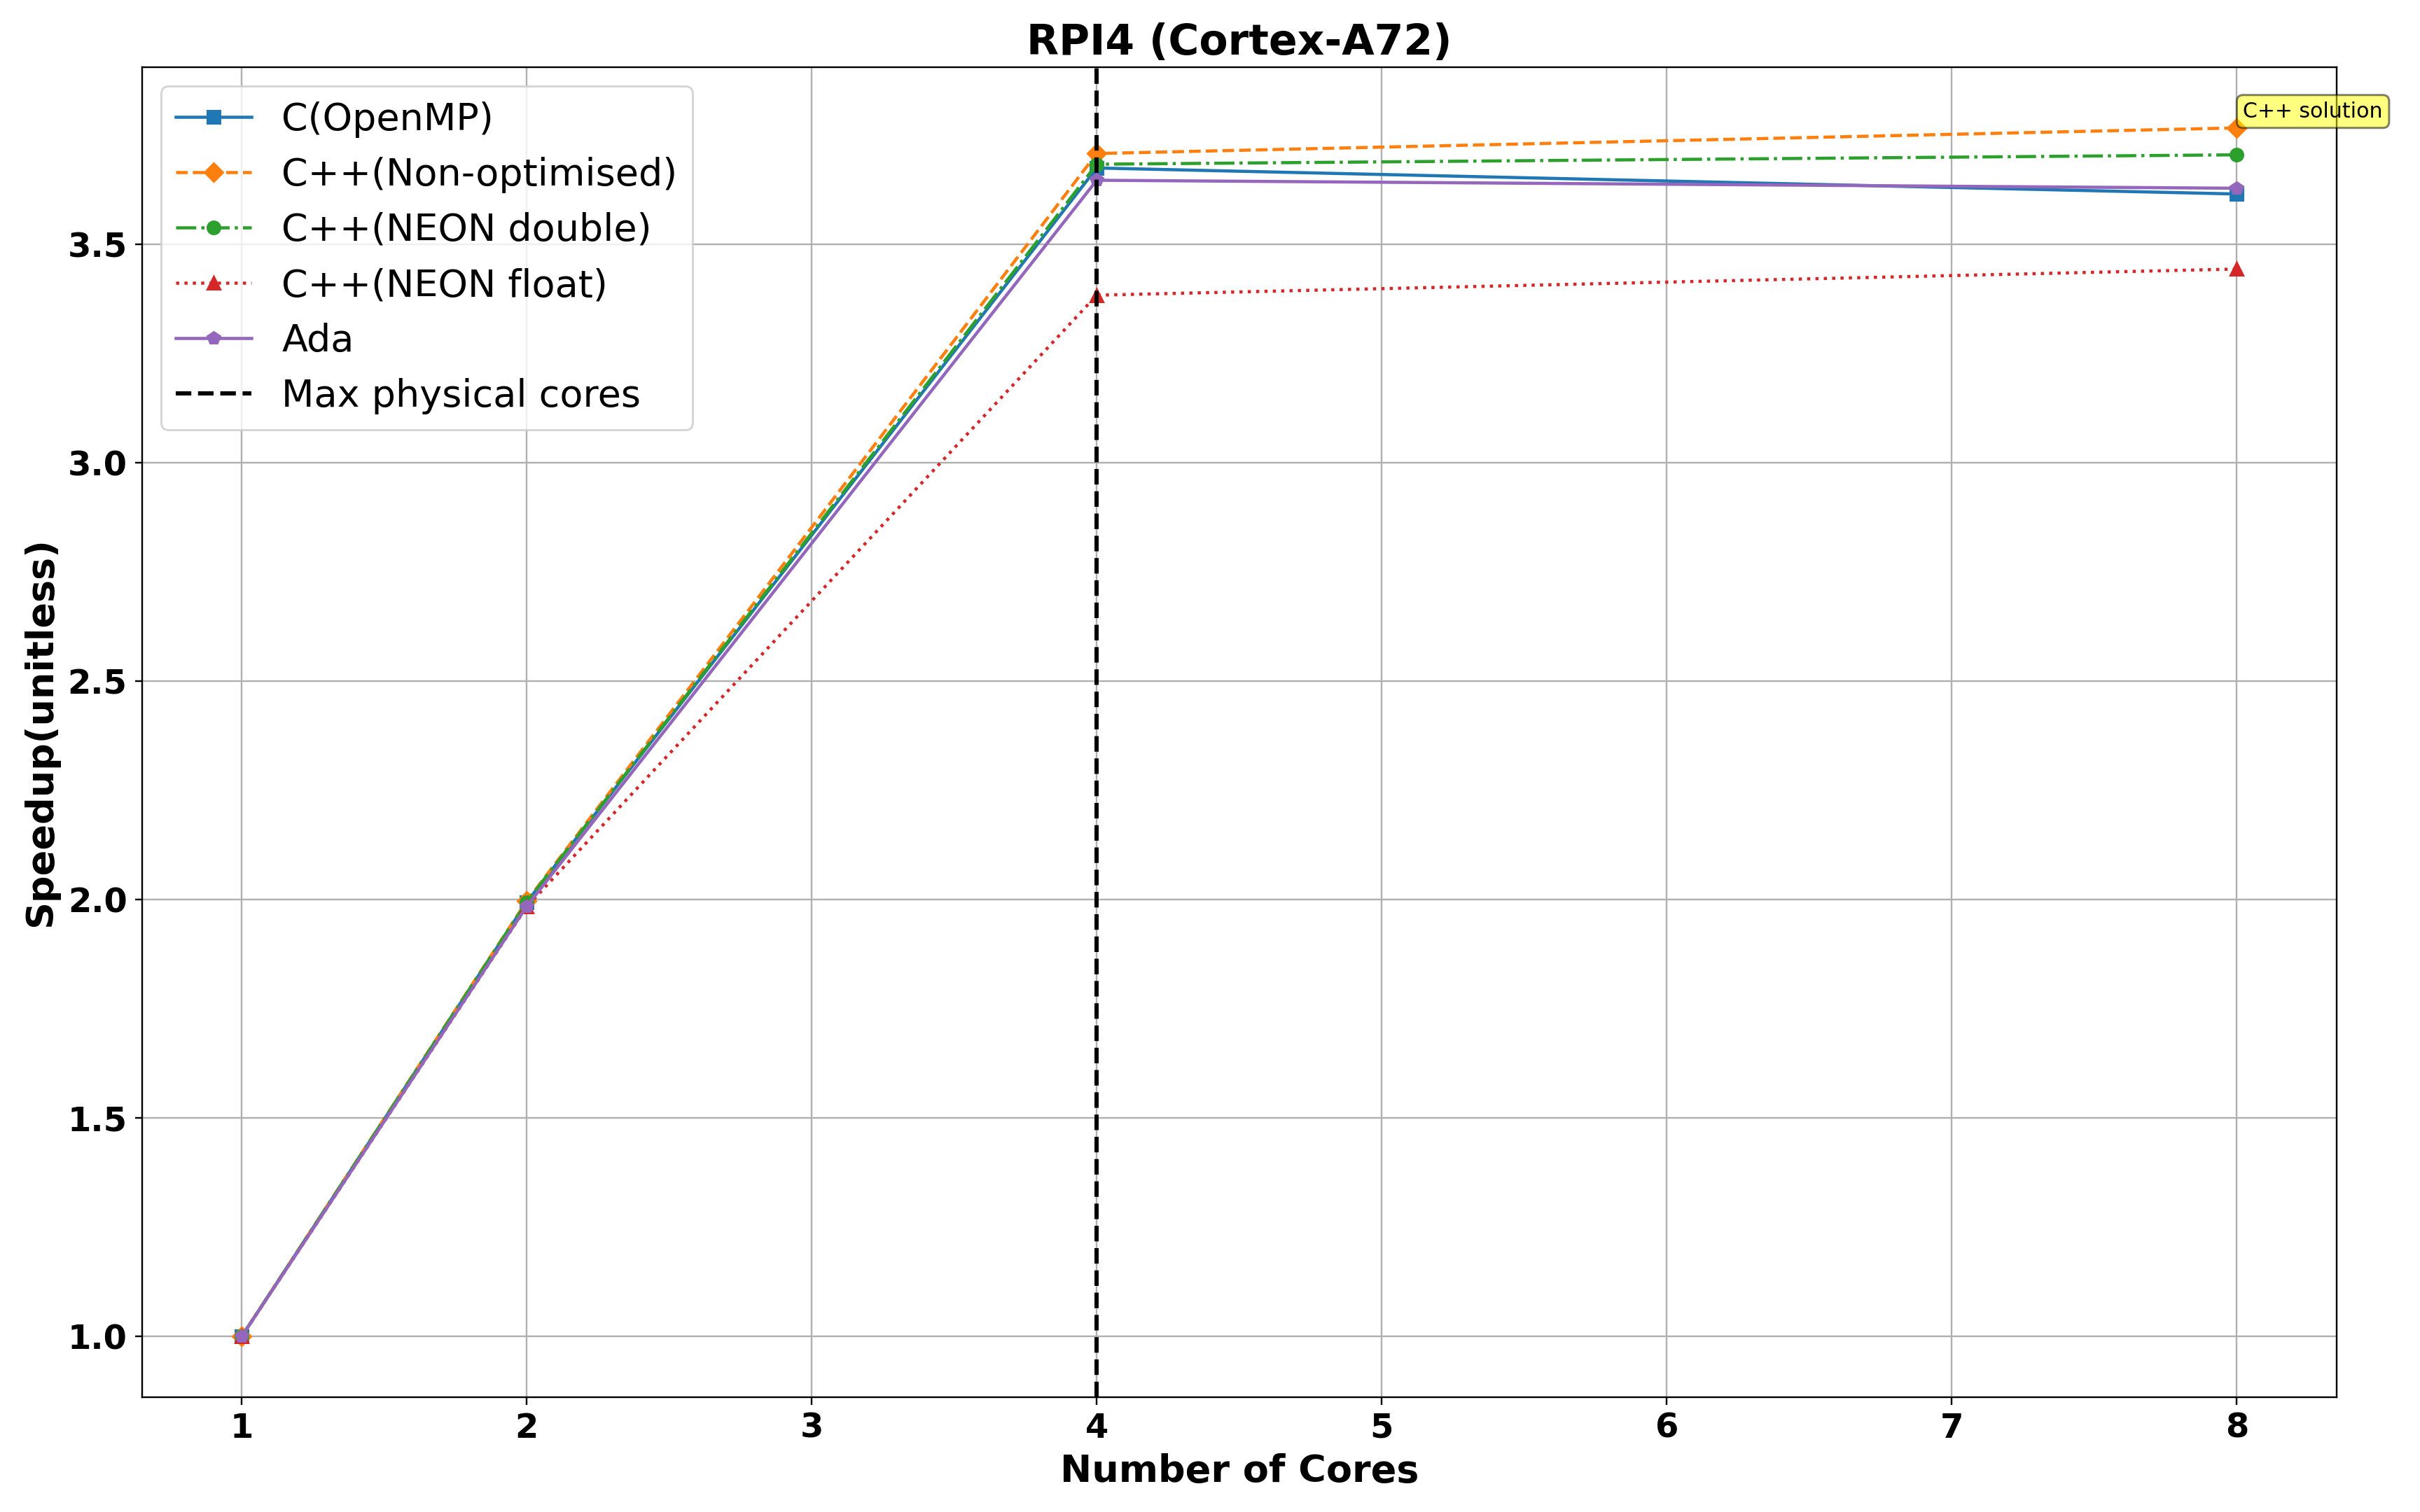
\includegraphics[width=1\textwidth, height=20cm]{~/Documents/Part_D_Modules/Individual_Project/Individual_report/figures/mpbenchmark_rpi4_speedup.png} % Adjust the path and width as needed
	\caption{Speedup plot collected from Raspberry Pi 4 processor. The vertical black line shows the maximum physical cores of the processor. (Higher is better).}
	\label{fig:mpbenchmark_rpi4_speedup_plot} % Use this label to reference the figure
\end{figure}

\section{Objective 2: \texttt{MobileNet}}

The \texttt{MobileNet} repository\cite{mobilenet_repo} contained some outdated portions of the code which were updated, certain parts of the code contained Chinese language which were translated into English and \texttt{CMake} build software was used to setup the \texttt{MobileNet} application. 

The main updates required to the original \texttt{MobileNet} repository\cite{mobilenet_repo} were inside the \texttt{readdata.cpp} file (listing ~\ref{lst:mobilenet_updates}). 

\begin{lstlisting}[
	caption={Updating the \texttt{ReadData::ReadInput()} function to use the latest \texttt{OpenCV} functions.},
	label={lst:mobilenet_updates}
	]
float* ReadData::ReadInput(const char* pcName) {
	std::cout << "Reading Picture: " << pcName << "..." << std::endl;
	
	// Use cv::Mat for image representation
	cv::Mat srcImage = cv::imread(pcName, cv::IMREAD_UNCHANGED);
	if (srcImage.empty()) {
		std::cerr << "Error: Image not loaded." << std::endl;
		return nullptr;
	}
	
	// Resize image
	cv::Mat dstImage;
	cv::resize(srcImage, dstImage, cv::Size(m_nInputWidth, m_nInputHeight), 0, 0, cv::INTER_LINEAR);
	
	int nOutputIndex = 0;
	
	for (int i = 0; i < dstImage.rows; i++) {
		for (int j = 0; j < dstImage.cols; j++) {
			nOutputIndex = i * m_nInputWidth + j;
			cv::Vec3b pixel = dstImage.at<cv::Vec3b>(i, j);
			m_pfInputData[nOutputIndex] = static_cast<float>(pixel[0]) - m_pfMean[nOutputIndex];
			m_pfInputData[nOutputIndex + m_nImageSize] = static_cast<float>(pixel[1]) - m_pfMean[nOutputIndex + m_nImageSize];
			m_pfInputData[nOutputIndex + 2 * m_nImageSize] = static_cast<float>(pixel[2]) - m_pfMean[nOutputIndex + 2 * m_nImageSize];
		}
	}
	
	std::cout << "Reading Picture Done..." << std::endl;
	
	return m_pfInputData;
}
\end{lstlisting}

The application was modified to have three command line arguments, this served primarily to make testing and collecting benchmark results easier for development purposes. The three arguments are as follows and can be seen in code in listing ~\ref{lst:mobilenet_command_line_arguments}:

\begin{enumerate}
	\item \texttt{test\_all}: This argument can be altered to either test one image or test all images in the data folder.  
	\item \texttt{write\_to\_file}: This argument is for writing benchmark data to a \texttt{.txt} file, this was useful for development purposes. It is recommended to leave this blank, so the project does not save any benchmark data. 
	\item \texttt{threads}: The number of threads that will be used by the application. It can be left blank to use the maximum number of available threads.  
\end{enumerate}

\begin{lstlisting}[
	caption={Altering the \texttt{MobileNet} application to use three command line arguments. \texttt{./mobilenet [test\_all] [write\_to\_file] [threads]}},
	label={lst:mobilenet_command_line_arguments}
	]
	int main(int argc, char* argv[])
	{
		//---------------------------Command line app logic
		bool testAllImages = false;
		bool writeDataToFile = false;  // Declare the variable to handle write to file logic
		bool g_DebugMode = true;       // Default debug mode setting
		int numThreads = 1;            // Default to 1 thread unless specified
		
		if (argc > 1) {
			std::string firstArg(argv[1]);
			testAllImages = (firstArg == "test_all");
		}
		if (argc > 2) {
			std::string secondArg(argv[2]);
			writeDataToFile = (secondArg == "write_to_file");
			g_DebugMode = !writeDataToFile; 
		}
		if (argc > 3) {
			numThreads = std::atoi(argv[3]);
			if (numThreads <= 0) {
				numThreads = omp_get_max_threads();  // Ensure OpenMP is included if used
			}
		}
		//--------------------------------------------------
		// Further logic and operations can follow here
	}
\end{lstlisting}


\texttt{Calgrind} profiling results from the \texttt{MobileNet} application show the following functions with the highest self-cost, these were \texttt{ConvLayer::forward}, \texttt{BatchNormalLayer::forward} and \texttt{ConvLayer::Addpad} as seen in figure ~\ref{fig:mobilenet_profiling}.

\begin{figure}[H] % Positioning preference: here, top, bottom, page
	\centering
	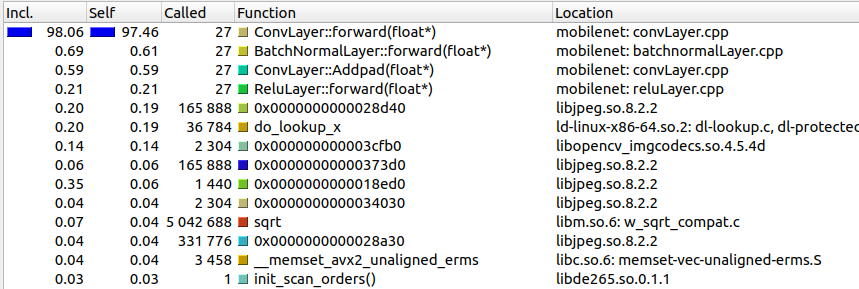
\includegraphics[width=1\textwidth, height=20cm]{~/Documents/Part_D_Modules/Individual_Project/Individual_report/figures/mobilenet_profiling.png} % Adjust the path and width as needed
	\caption{\texttt{Calgrind} profiling results, functions with the highest self-cost.}
	\label{fig:mobilenet_profiling} % Use this label to reference the figure
\end{figure}


The parallelisation of functions \texttt{BatchNormalLayer::forward} and \texttt{ConvLayer::Addpad} can be found in listings ~\ref{lst:mobilenet_function1_parallel} and ~\ref{lst:mobilenet_function2_parallel}.

\begin{lstlisting}[
	caption={Parallelising the \texttt{BatchNormalLayer::forward()} function.},
	label={lst:mobilenet_function1_parallel}
	]
void BatchNormalLayer::forward(float *pfInput) 
{
	#pragma omp parallel for collapse(2) shared(m_nInputNum, m_nInputSize, pfInput, m_pfOutput, m_pfFiller, m_pfMean, m_pfVar, m_pfBias) 
	for (int i = 0; i < m_nInputNum; i++)
	{
		for (int j = 0; j < m_nInputSize; j++)
		{
			int nOutputIndex = i * m_nInputSize + j;
			
			m_pfOutput[nOutputIndex] = m_pfFiller[i] * ((pfInput[nOutputIndex] - m_pfMean[i])
			/ sqrt(m_pfVar[i] + 1e-5)) + m_pfBias[i];
		}
	}
}
\end{lstlisting}


\begin{lstlisting}[
	caption={Parallelising the \texttt{ConvLayer::Addpad()} function If the \texttt{EMBEDDED\_PROC} is not set.},
	label={lst:mobilenet_function2_parallel}
	]
void ConvLayer::Addpad(float *pfInput)
{
	// Only use OpenMP pragmas if EMBEDDED_PROC is not defined, such as on a laptop/desktop CPU 
	#ifndef EMBEDDED_PROC
	#pragma omp parallel for collapse(2)
	#endif
	for (int m = 0; m < m_nInputNum; m++)
	{
		for (int i = 0; i < m_nInputPadWidth; i++)
		{
			for (int j = 0; j < m_nInputPadWidth; j++)
			{
				if ((i < m_nPad) || (i >= m_nInputPadWidth - m_nPad))
				{
					m_pfInputPad[m * m_nInputPadSize + i * m_nInputPadWidth + j] = 0;
				}
				else if ((j < m_nPad) || (j >= m_nInputPadWidth - m_nPad))
				{
					m_pfInputPad[m * m_nInputPadSize + i * m_nInputPadWidth + j] = 0;
				}
				else
				{
					m_pfInputPad[m * m_nInputPadSize + i * m_nInputPadWidth + j] = pfInput[m * m_nInputSize + (i - m_nPad) * m_nInputWidth + (j - m_nPad)];
				}
			}
		}
	}
}
\end{lstlisting}

% Addition of command line arguments
% Valgrind results 
% All the parallelised code

Results collected from Raspberry Pi 4 can be seen in figures ~\ref{fig:mobilenet_rpi4_plot} and ~\ref{fig:mobilenet_rpi4_speedup}. 

\begin{figure}[H] % Positioning preference: here, top, bottom, page
	\centering
	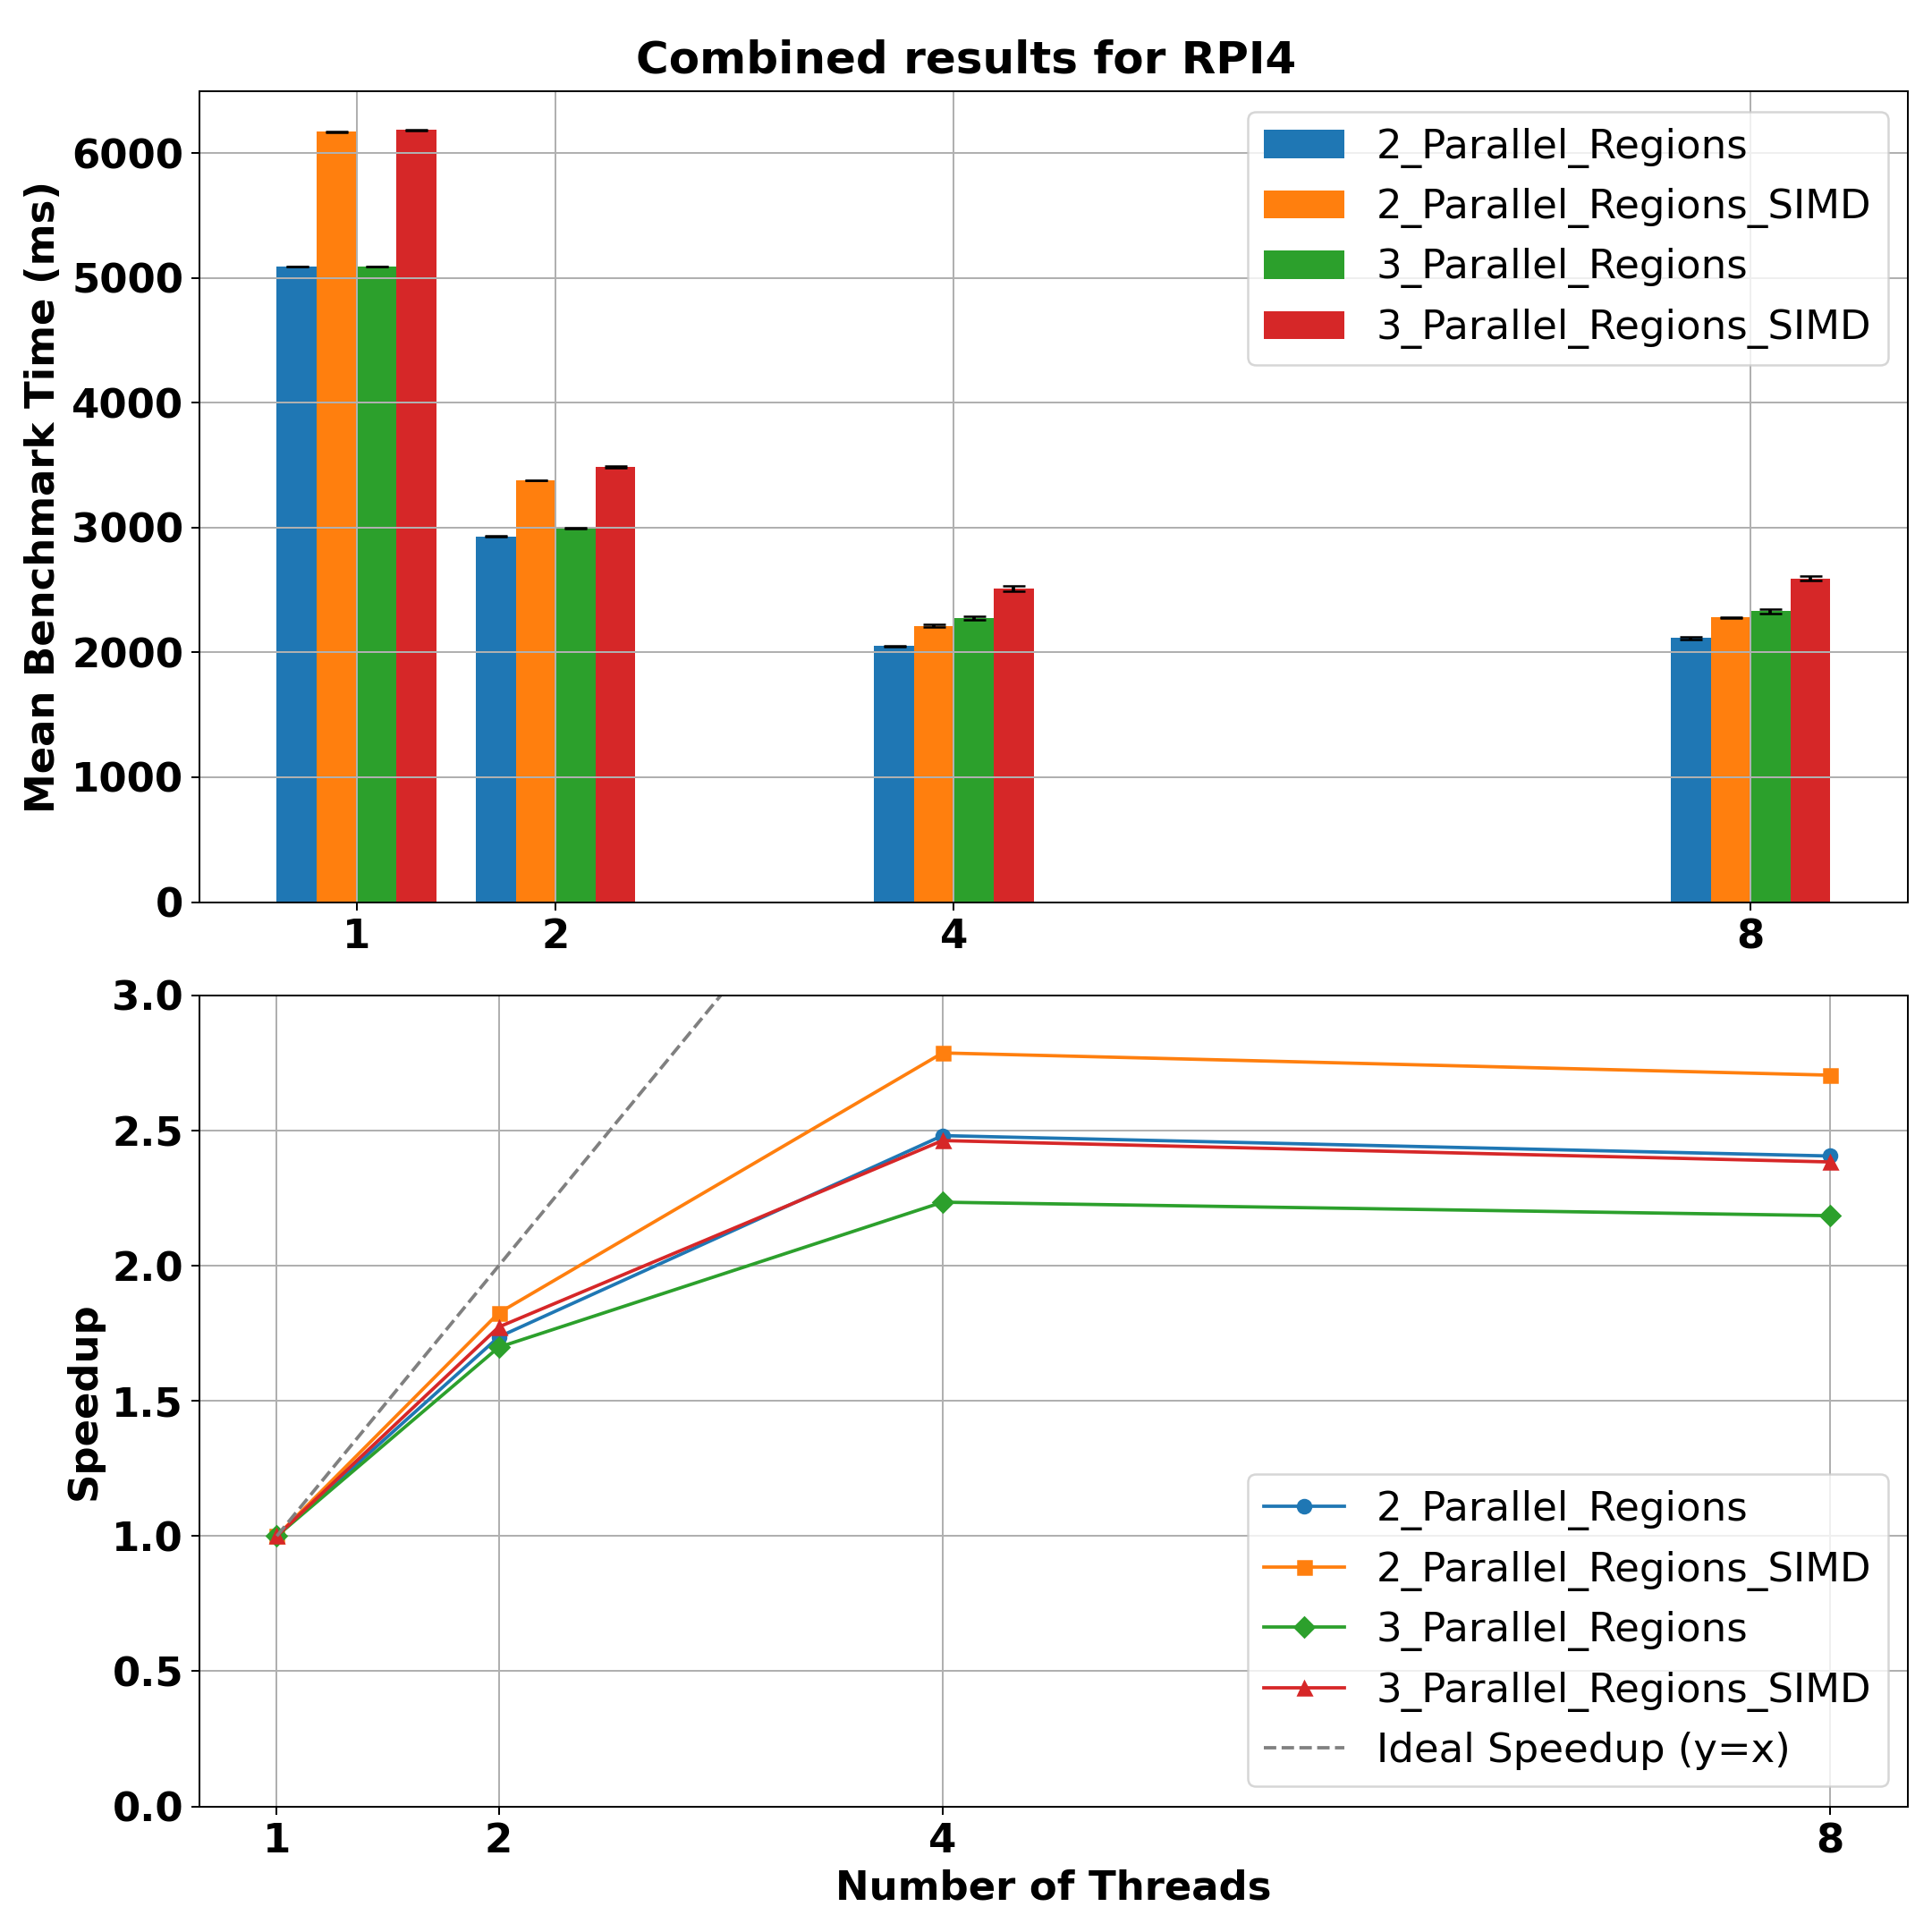
\includegraphics[width=1\textwidth, height=20cm]{~/Documents/Part_D_Modules/Individual_Project/Individual_report/figures/mobilenet_rpi4.png} % Adjust the path and width as needed
	\caption{Mean benchmark plot of results collected from \texttt{Cortex A-72} processor(in milliseconds). (Lower is better).}
	\label{fig:mobilenet_rpi4_plot} % Use this label to reference the figure
\end{figure}

\begin{figure}[H] % Positioning preference: here, top, bottom, page
	\centering
	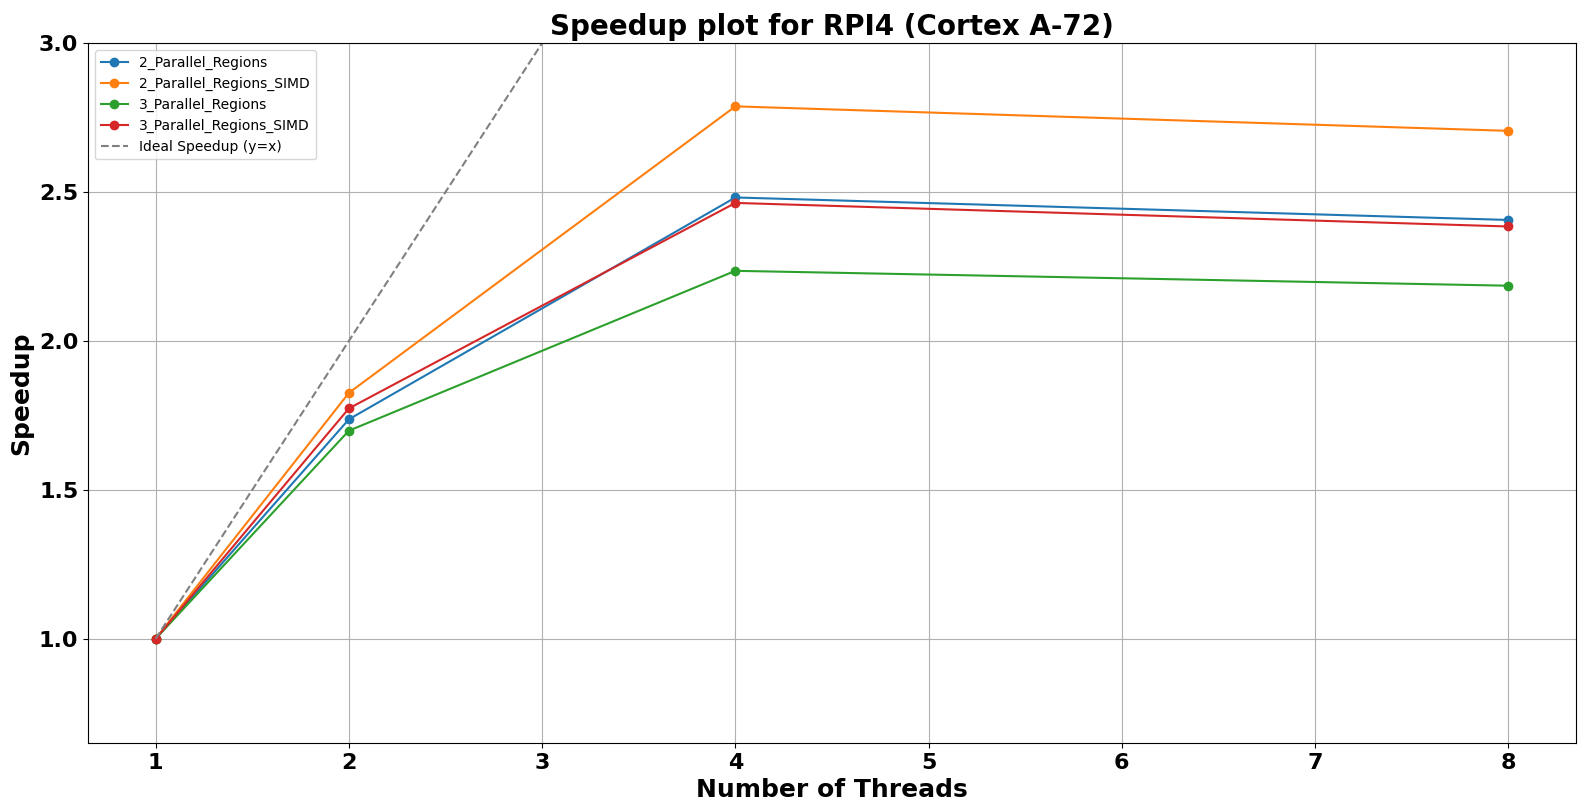
\includegraphics[width=1\textwidth, height=20cm]{~/Documents/Part_D_Modules/Individual_Project/Individual_report/figures/mobilenet_rpi4_speedup.png} % Adjust the path and width as needed
	\caption{Speedup plot comparing different solutions with results collected from \texttt{Cortex A-72} processor. (Higher is better).}
	\label{fig:mobilenet_rpi4_speedup} % Use this label to reference the figure
\end{figure}

\section{Objective 3: \texttt{DeBaTE-FI} platform}

The application was profiled using \texttt{py-spy} tool. The application spawned multiple processes, therefore they were profiled separately. Profiling results from the process responsible for the GUI of the application are shown in figure ~\ref{fig:debate_profile_1} and the profiling results from the process responsible for communicating with the MCUs are shown in figure ~\ref{fig:debate_profile_2}.

\begin{figure}[H] % Positioning preference: here, top, bottom, page
	\centering
	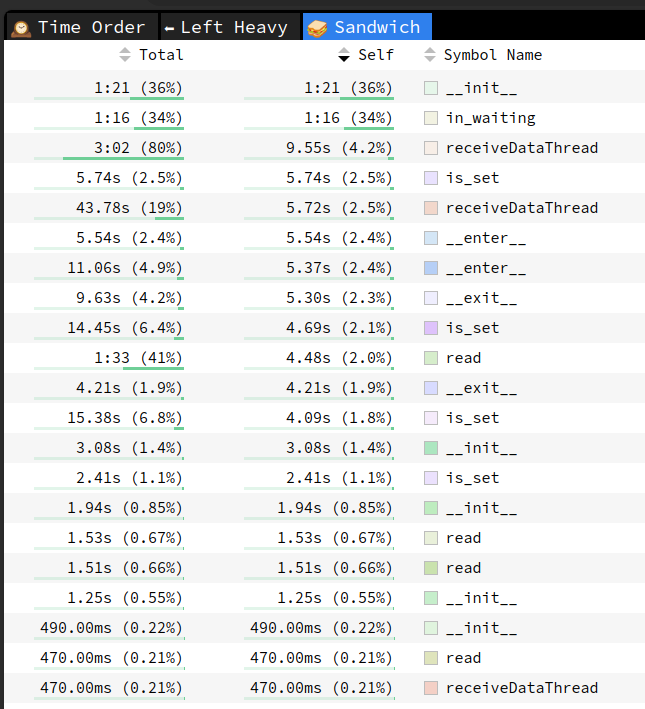
\includegraphics[width=1\textwidth, height=20cm]{~/Documents/Part_D_Modules/Individual_Project/Individual_report/figures/debate_fi_platform_app.png} % Adjust the path and width as needed
	\caption{Profiling results for the application GUI process visualised in \texttt{speedscope} web application\cite{speedscope_app}. }
	\label{fig:debate_profile_1} % Use this label to reference the figure
\end{figure}

\begin{figure}[H] % Positioning preference: here, top, bottom, page
	\centering
	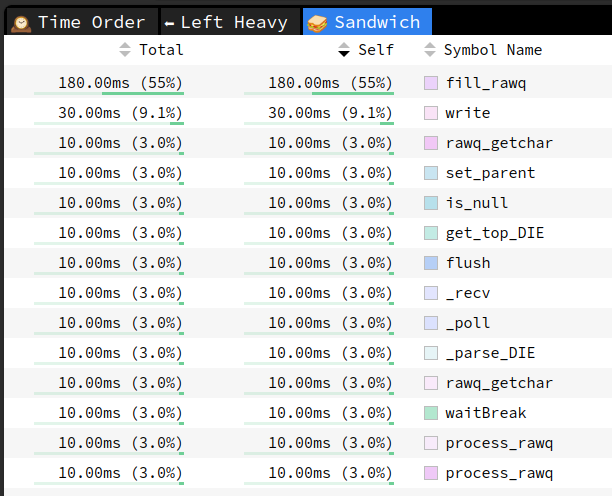
\includegraphics[width=1\textwidth, height=20cm]{~/Documents/Part_D_Modules/Individual_Project/Individual_report/figures/debate_fi_platform_openocd.png} % Adjust the path and width as needed
	\caption{Profiling results for the \texttt{OpenOCD/telnet} process visualised in \texttt{speedscope} web application\cite{speedscope_app}.}
	\label{fig:debate_profile_2} % Use this label to reference the figure
\end{figure}


%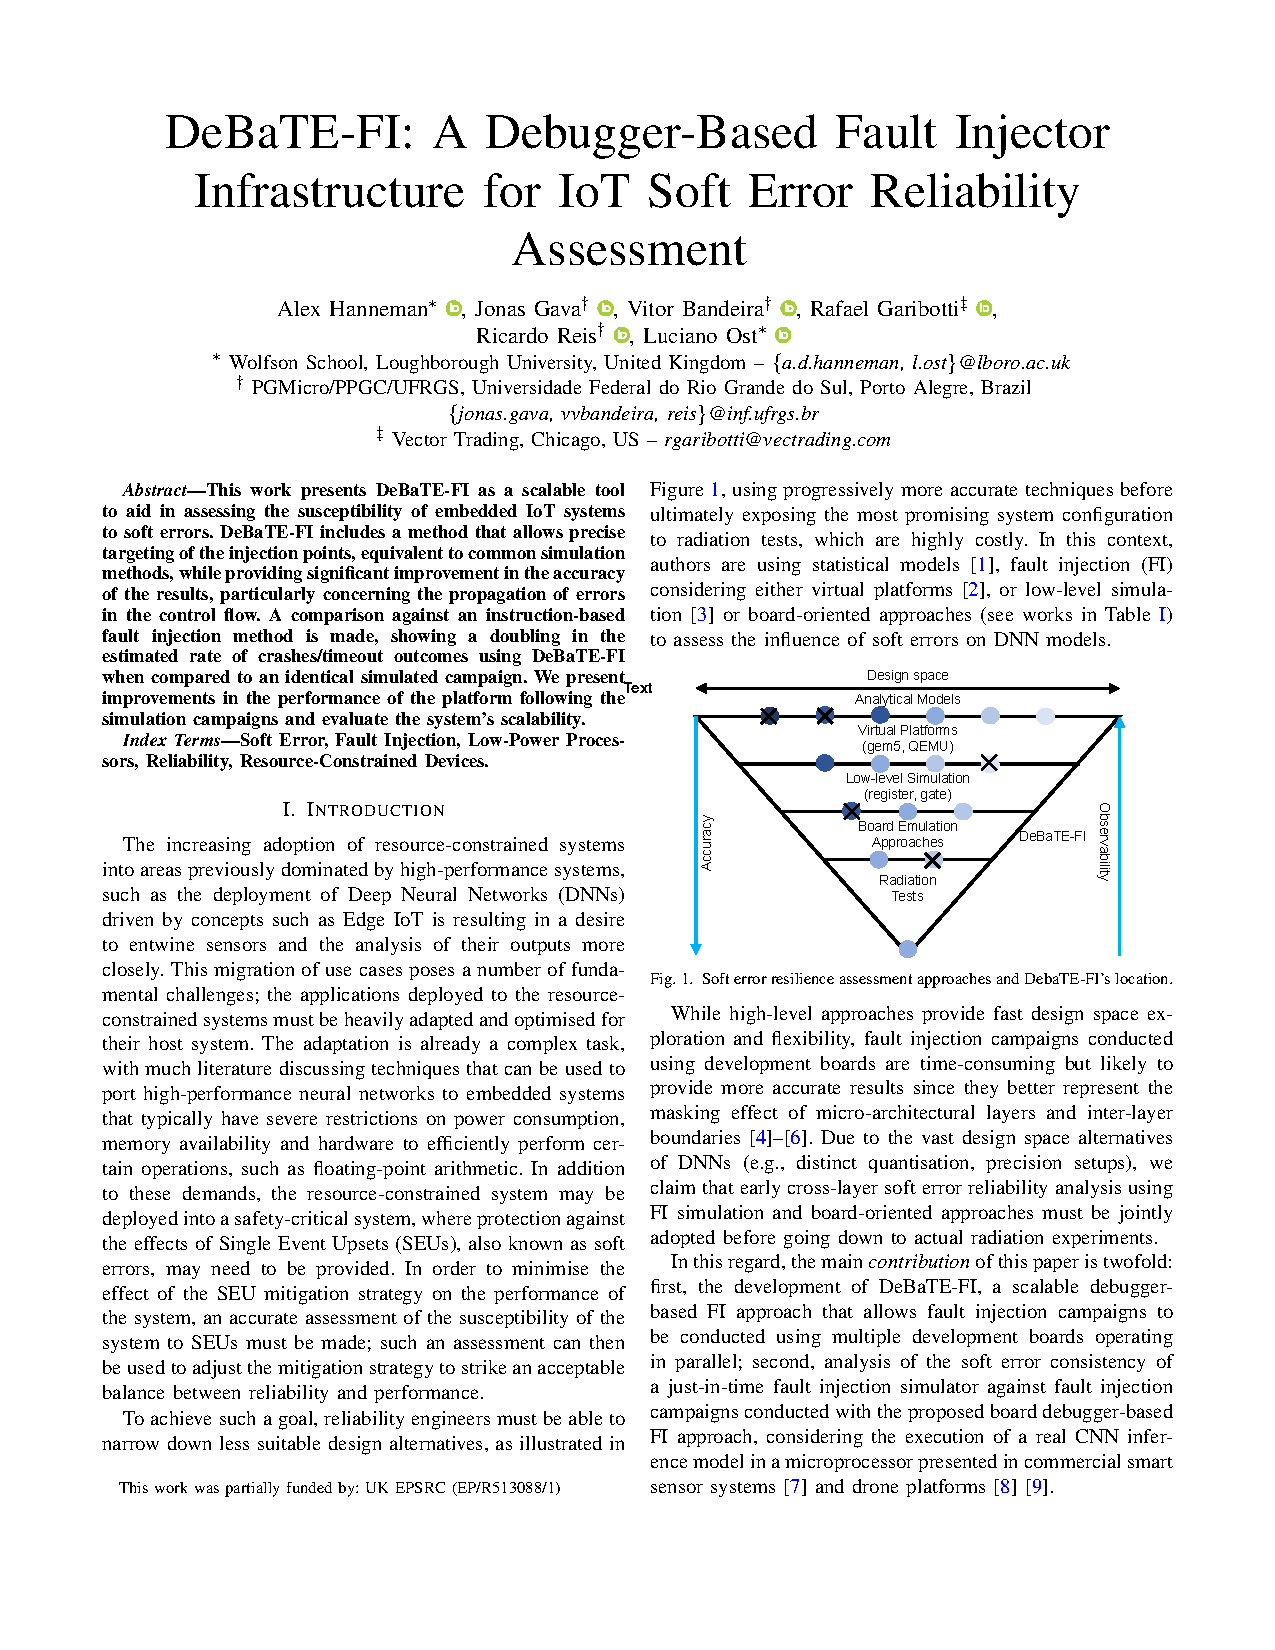
\includepdf[
%pages=-,
%addtotoc={1, section, 1, DeBaTE-FI platform publication(maybe remove?), appendix:debate_fi},
%pagecommand={\label{appendix:debate_fi}}
%]{~/Documents/Part_D_Modules/Individual_Project/Individual_report/files/Debate_FI_platform.pdf}


